\subsection{Algorithme de Ritter}
Le dernier algorithme utilisé que nous allons présenter et celui de Jack Ritter en 1990 et permet de calculer le cercle minimum. C'est un algorithme glouton, en d'autres mots, l'algorithme retourne une bonne solution mais pas la plus optimale contrairement à un algorithme naïf. En revanche, la perte d'efficacité est gagné en complexité qui s'avère beaucoup plus rapide puisque qu'elle se fait complexité linéaire en la taille de l'entrée $\mathcal{O}(n)$.

\begin{figure}[ht]
\begin{center}
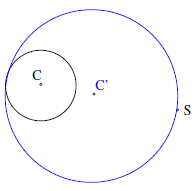
\includegraphics[scale=0.9]{images/ritter.png}
\caption{Algorithme de Ritter}
\end{center}
\end{figure}

L'idée est d'agrandir progressivement le cercle afin de couvrir tous les points de l'ensemble. La description de l'algorithme est donné ci-dessous par  (voir référence \cite{cpa}) :

\begin{enumerate}
\item Prendre un point $dummy$ quelconque appartenant à l'ensemble des points de départ.
\item Parcourir l'ensemble des points pour trouver un point $P$ de distance maximum au point $dummy$.
\item Reparcourir l'ensemble des points pour trouver un point $Q$ de distance maximum au point P.
\item Considérer le point $C$, le centre du segment $PQ$.
\item Considérer le cercle $CERCLE$ centré en $C$, de rayon $\lvert CP \rvert$ : il passe par $P$ et $Q$.
\item Retirer les points $P$ et $Q$ de l'ensemble des points.
\item Tant qu'il reste des points dans l'ensemble, considérer un point $S$ quelconque.
\item Si $S$ est couvert par $CERCLE$, retirer $S$ de l'ensemble des points; répéter l'étape 7.
\item Sinon, tracer au brouillon la droite passant par $S$ et $C$. Celle-ci coupe le périmètre du cercle courant en deux points : soit $T$ le point le plus eloigné de $S$.
\item Déterminer les coordonnées du point $C'$, le centre du segment $ST$.
\item Remplacer $CERCLE$ par le cercle centré en $C$, de rayon $\lvert C'T \rvert$ : il passe par $S$ et $T$.
\item. Repéter 'étape 7. jusqu'à ce qu'il ne reste plus de points dans la liste.
\end{enumerate}

\begin{figure}[ht]
\begin{center}
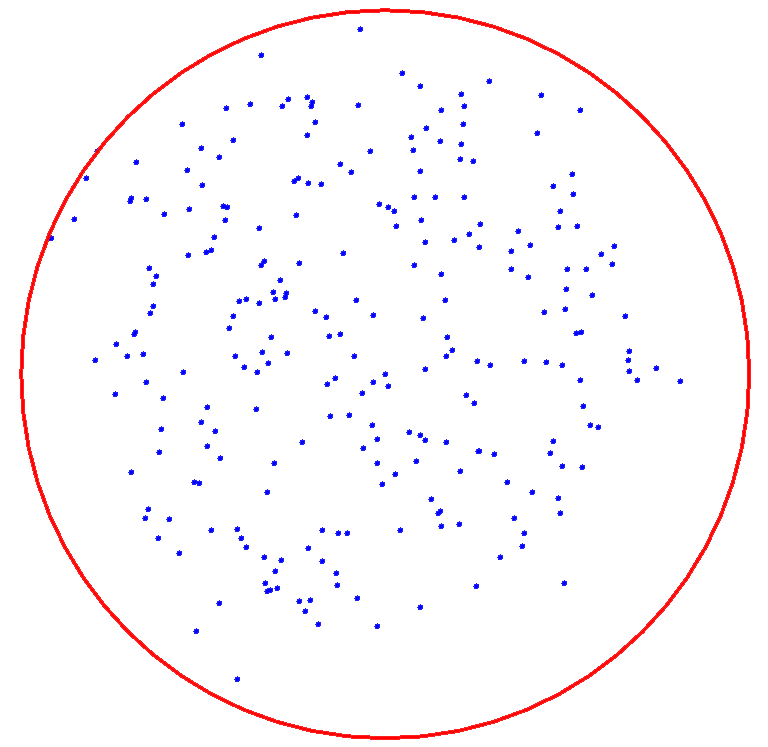
\includegraphics[scale=0.25]{images/ex_ritter.png}
\caption{Exemple d'application Ritter}
\end{center}
\end{figure}